\documentclass[10pt,letterpaper, landscape]{article}
\usepackage[table]{xcolor}
\definecolor{lightgray}{gray}{0.85}
\usepackage[utf8]{inputenc}
\usepackage{scalefnt}
\usepackage{amsmath}
\usepackage{amsfonts}
\usepackage{amssymb}
\usepackage{graphicx}
\usepackage{textcomp}
\usepackage[left=0.25in, right=0.25in, top=0.25in, bottom=.25in]{geometry}
%\geometry{paperwidth=15.125in,paperheight=11.6875in}
%\setlength{\paperwidth}{15.125in}
%\setlength{\paperheight}{11.6875in}

\usepackage{url}

\usepackage{multicol}

\newcounter{NumberInTable}
\newcommand{\NUM}{\stepcounter{NumberInTable}{(\theNumberInTable)}}
%\newcommand{\Formula}[2]{{#1}\>{\ensuremath{\displaystyle{#2}}}\>\NUM}
%\newcommand{\MFormula}[2]{{\begin{minipage}{1.5in}#1\end{minipage}}\>{\ensuremath{\displaystyle{#2}}}\>\NUM}

\newcommand{\Formula}[2]{{#1}{\begin{align}{\displaystyle{#2}}\end{align}}}


\newcommand{\SETTABS}{\hspace*{2in}\=\hspace{4.in}\=\kill}

\begin{document}
\thispagestyle{empty}
\setlength{\parindent}{0pt}
\setlength{\columnseprule}{0.4pt}
\setlength{\columnsep}{3ex}

{\LARGE \begin{center}
\textbf{Basic Statistics  Formulas}
\end{center}}
\begin{multicols}{3}
{\large \textbf{Population Measures}}
\begin{align}
\text{Mean } \mu &= \dfrac{1}{n}\sum x_i\\
\text{Variance } \sigma^2 &= \dfrac{1}{n}\sum(x_i-\overline{x})^2\\
\text{Standard Deviation } \sigma&=\sqrt{\dfrac{1}{n}\sum(x_i-\overline{x})^2}
\end{align}
\hrulefill

{\large \textbf{Sampling}}
\begin{align}
\text{Sample mean } \overline{x} &= \dfrac{1}{n}\sum x_i\\
\text{Sample variance } s_x^2 &= \dfrac{1}{n-1}\sum(x_i-\overline{x})^2\\
\text{Std. Deviation } s_x&=\sqrt{\dfrac{1}{n-1}\sum(x_i-\overline{x})^2}\\
\text{z-score }z&=\dfrac{x-\mu}{\sigma}\\
\text{Correlation }r&=\nonumber \\
\dfrac{1}{n-1}\sum_{i=1}^n &\left(\dfrac{(x_i-\overline{x})}{s_x} \right) \left(\dfrac{(y_i-\overline{y})}{s_y} \right)
\end{align}

\hrulefill

{\large \textbf{Linear Regression}}
\begin{align}
\text{Line } \hat{y}&=a+bx \\
b&=r\dfrac{s_y}{s_x}, 
a=\overline{y}-b\overline{x}  \\
s &=\sqrt{\dfrac{1}{n-2}{\sum_{i=1}^n(y_i-\hat{y})^2}}\\
SE_b &=\dfrac{s}{\sqrt{\displaystyle{\sum_{i=1}^n\left (x_i-\overline{x}\right )^2}}}\\
\text{To test } & H_0:b=0, \text{ use }t = \dfrac{b}{SE_b} \\
CI &= b \pm t^* SE_b
\end{align}


%\columnbreak

{\large \textbf{Probability}}
\begin{align}
P(A\text{ or } B)&=P(A)+P(B)-P(A\text{ and }B)\\
P(\text{not }A)&=1-P(A)\\
P(A\text{ and }B)&=P(A)P(B)\text{ (independent)} \\
P(B|A)&=P(A\text{ and } B)/{P(A)}\\
0!=1; 
n! &= 1\times 2 \times 3 \cdots \times (n-1)\times n\\
\binom{n}{k}&=\dfrac{n!}{k!(n-k)!}\\
\text{Binomial Dist}&\text{ribution}:\nonumber\\
P(\mathcal{X}&=k)=\binom{n}{k}p^k(1-p)^{n-k}\\
\mu&=np, \ \sigma = \sqrt{np(1-p)}
\end{align}




\hrulefill

{\large \textbf{One-Sample z-statistic}}
\begin{align}
\text{To test } H_0: \mu=\mu_0\text{ use} 
z &= \dfrac{\overline{z}-\mu_0}{\sigma/\sqrt{n}}\\
\text{Confidence Interval for }\mu &= \overline{x}\pm z^* \dfrac{\sigma}{\sqrt{n}}\\
\text{Margin of Error }ME &=z^* \dfrac{\sigma}{\sqrt{n}}\\
\text{Minimum sample size }n &\geq \left[ \dfrac{z^*\sigma}{ME}\right]^2
\end{align}
\hrulefill

{\large \textbf{One-Sample t-statistic}}
\begin{align}
 SEM &=\dfrac{s_x}{\sqrt{n}}, 
\ t=\dfrac{\overline{x}-\mu}{s_x/\sqrt{n}}\\
\text{Confidence Interval} &= \overline{x}\pm t^*\dfrac{s_x}{\sqrt{n}}
\end{align}
\hrulefill

{\large \textbf{Two-Sample t-statistic}}
\begin{align}
t&=\dfrac{\overline{x}_1 -\overline{x}_2}{
\sqrt{\dfrac{s_1^2}{n_1}+\dfrac{s_2^2}{n_2}}}\\ 
\text{Conf. Interval}&=
(\overline{x}_1-\overline{x}_2)\pm t^*\sqrt{\dfrac{s_1^2}{n_1}+\dfrac{s_2^2}{n_2}}
\end{align}

%\columnbreak

{\large \textbf{Sample Proportions}}
\begin{align}
\mu_{\hat{p}} &=p, \
\sigma_{\hat{p}} = \sqrt{\dfrac{p(1-p)}{n}}\\
\text{Conf. Int.} &= \hat{p}\pm z^*(SE)\\
\text{SE} &=\sqrt{\dfrac{\hat{p}(1-\hat{p})}{n}}\\
\text{sample size } n &> \left[\dfrac{z^*}{ME}\right]^2 p^*(1-p^*)\\
\text{To test } H_0:p=p_0, \text{ use }  
z &= \dfrac{\hat{p}-p_0}{\sqrt{\dfrac{p_0(1-p_0)}{n}}}
\end{align}
\hrulefill

{\large \textbf{Two-Sample Proportions}}
\begin{align}
SE &= \sqrt{\dfrac{\hat{p}_1(1-\hat{p}_1)}{n_1} + \dfrac{\hat{p}_2(1-\hat{p}_2)}{n_2}}\\
CI &= (\hat{p}_1-\hat{p}_2)\pm z^* (SE)\\
\text{To test }&H_0: p_1=p_2, \text{ use}\\
z&=\dfrac{\hat{p}_1-\hat{p}_2}{\sqrt{\hat{p}(1-\hat{p})\left(\dfrac{1}{n_1}+\dfrac{1}{n_2}\right)}} \\
\hat{p}&=\dfrac{X_1 + X_2}{n_1 + n_2}, \ X_i = \text{ successes}
\end{align}
\hrulefill

{\large \textbf{Chi-Square Statistic}}
\begin{align}
\chi^2 &= \sum_{i=1}^n\dfrac{(o_i-e_i)^2}{e_i}\\
o_i&=\text{observed}\nonumber,
 e_i=\text{expected}\nonumber
\end{align}

\hrulefill

\Formula{\large \textbf{Central Limit Theorem}}
{
s_{\overline{x}} \to \dfrac{\sigma}{\sqrt{n}} \text{ as  } n\to \infty
} 
 
\end{multicols}
\hrulefill


{\footnotesize \textcopyleft\ 2013 B.E. Shapiro. This work is licensed under a \textit{{Creative Commons Attribution-NonCommercial-ShareAlike 3.0 Unported License}} (BY-NC-SA 3.0). See \url{http://creativecommons.org/licenses/by-nc-sa/3.0/} for details. Please address all corrections to \url{bruce.e.shapiro@csun.edu}. Last revised \today. \ Original PDF and \LaTeX\ files available at  \url{http://integral-table.com/}}
\begin{center}
\begin{minipage}{5in}
\begin{flushright}
\begin{minipage}{2.25in}
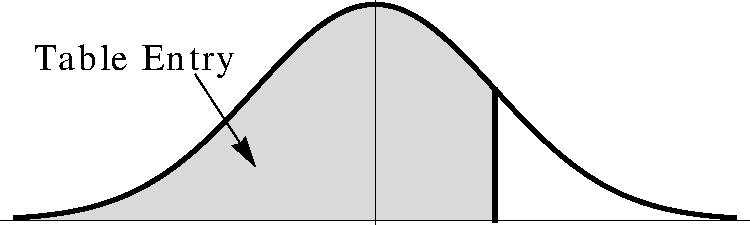
\includegraphics[width=.75\textwidth]{Normal-Curve.pdf} \\
\sffamily
\scalefont{.5} Standard Normal Cumulative Proportions (below)
\end{minipage}%\hfill
\begin{minipage}{2.25in} 
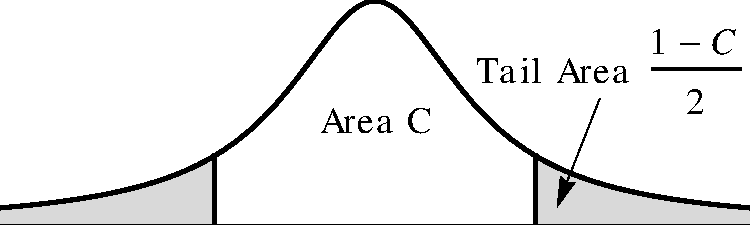
\includegraphics[width=.75\textwidth]{t-Curve.pdf}\\
\sffamily\scalefont{.5}t-Distribution Critical Values (to right)
\end{minipage}
\end{flushright}
\begin{center}
Standard Normal Cumulative Proportions
\sffamily
\scalefont{.5}
\renewcommand{\arraystretch}{1.1}
\begin{tabular}{|r|rrrrrrrrrr|}
\hline		&	0	&	0.01	&	0.02	&	0.03	&	0.04	&	0.05	&	0.06	&	0.07	&	0.08	&	0.09	\\ \hline
	-3.4	&	0.0003	&	0.0003	&	0.0003	&	0.0003	&	0.0003	&	0.0003	&	0.0003	&	0.0003	&	0.0003	&	0.0002	\\
	-3.3	&	0.0005	&	0.0005	&	0.0005	&	0.0004	&	0.0004	&	0.0004	&	0.0004	&	0.0004	&	0.0004	&	0.0003	\\
	-3.2	&	0.0007	&	0.0007	&	0.0006	&	0.0006	&	0.0006	&	0.0006	&	0.0006	&	0.0005	&	0.0005	&	0.0005	\\
	-3.1	&	0.0010	&	0.0009	&	0.0009	&	0.0009	&	0.0008	&	0.0008	&	0.0008	&	0.0008	&	0.0007	&	0.0007	\\
	-3	&	0.0013	&	0.0013	&	0.0013	&	0.0012	&	0.0012	&	0.0011	&	0.0011	&	0.0011	&	0.0010	&	0.0010	\\
\cellcolor{lightgray}	-2.9	&\cellcolor{lightgray}	0.0019	&\cellcolor{lightgray}	0.0018	&\cellcolor{lightgray}	0.0018	&\cellcolor{lightgray}	0.0017	&\cellcolor{lightgray}	0.0016	&\cellcolor{lightgray}	0.0016	&\cellcolor{lightgray}	0.0015	&\cellcolor{lightgray}	0.0015	&\cellcolor{lightgray}	0.0014	&\cellcolor{lightgray}	0.0014	\\
\cellcolor{lightgray}	-2.8	&\cellcolor{lightgray}	0.0026	&\cellcolor{lightgray}	0.0025	&\cellcolor{lightgray}	0.0024	&\cellcolor{lightgray}	0.0023	&\cellcolor{lightgray}	0.0023	&\cellcolor{lightgray}	0.0022	&\cellcolor{lightgray}	0.0021	&\cellcolor{lightgray}	0.0021	&\cellcolor{lightgray}	0.0020	&\cellcolor{lightgray}	0.0019	\\
\cellcolor{lightgray}	-2.7	&\cellcolor{lightgray}	0.0035	&\cellcolor{lightgray}	0.0034	&\cellcolor{lightgray}	0.0033	&\cellcolor{lightgray}	0.0032	&\cellcolor{lightgray}	0.0031	&\cellcolor{lightgray}	0.0030	&\cellcolor{lightgray}	0.0029	&\cellcolor{lightgray}	0.0028	&\cellcolor{lightgray}	0.0027	&\cellcolor{lightgray}	0.0026	\\
\cellcolor{lightgray}	-2.6	&\cellcolor{lightgray}	0.0047	&\cellcolor{lightgray}	0.0045	&\cellcolor{lightgray}	0.0044	&\cellcolor{lightgray}	0.0043	&\cellcolor{lightgray}	0.0041	&\cellcolor{lightgray}	0.0040	&\cellcolor{lightgray}	0.0039	&\cellcolor{lightgray}	0.0038	&\cellcolor{lightgray}	0.0037	&\cellcolor{lightgray}	0.0036	\\
\cellcolor{lightgray}	-2.5	&\cellcolor{lightgray}	0.0062	&\cellcolor{lightgray}	0.0060	&\cellcolor{lightgray}	0.0059	&\cellcolor{lightgray}	0.0057	&\cellcolor{lightgray}	0.0055	&\cellcolor{lightgray}	0.0054	&\cellcolor{lightgray}	0.0052	&\cellcolor{lightgray}	0.0051	&\cellcolor{lightgray}	0.0049	&\cellcolor{lightgray}	0.0048	\\
	-2.4	&	0.0082	&	0.0080	&	0.0078	&	0.0075	&	0.0073	&	0.0071	&	0.0069	&	0.0068	&	0.0066	&	0.0064	\\
	-2.3	&	0.0107	&	0.0104	&	0.0102	&	0.0099	&	0.0096	&	0.0094	&	0.0091	&	0.0089	&	0.0087	&	0.0084	\\
	-2.2	&	0.0139	&	0.0136	&	0.0132	&	0.0129	&	0.0125	&	0.0122	&	0.0119	&	0.0116	&	0.0113	&	0.0110	\\
	-2.1	&	0.0179	&	0.0174	&	0.0170	&	0.0166	&	0.0162	&	0.0158	&	0.0154	&	0.0150	&	0.0146	&	0.0143	\\
	-2	&	0.0228	&	0.0222	&	0.0217	&	0.0212	&	0.0207	&	0.0202	&	0.0197	&	0.0192	&	0.0188	&	0.0183	\\
\cellcolor{lightgray}	-1.9	&\cellcolor{lightgray}	0.0287	&\cellcolor{lightgray}	0.0281	&\cellcolor{lightgray}	0.0274	&\cellcolor{lightgray}	0.0268	&\cellcolor{lightgray}	0.0262	&\cellcolor{lightgray}	0.0256	&\cellcolor{lightgray}	0.0250	&\cellcolor{lightgray}	0.0244	&\cellcolor{lightgray}	0.0239	&\cellcolor{lightgray}	0.0233	\\
\cellcolor{lightgray}	-1.8	&\cellcolor{lightgray}	0.0359	&\cellcolor{lightgray}	0.0351	&\cellcolor{lightgray}	0.0344	&\cellcolor{lightgray}	0.0336	&\cellcolor{lightgray}	0.0329	&\cellcolor{lightgray}	0.0322	&\cellcolor{lightgray}	0.0314	&\cellcolor{lightgray}	0.0307	&\cellcolor{lightgray}	0.0301	&\cellcolor{lightgray}	0.0294	\\
\cellcolor{lightgray}	-1.7	&\cellcolor{lightgray}	0.0446	&\cellcolor{lightgray}	0.0436	&\cellcolor{lightgray}	0.0427	&\cellcolor{lightgray}	0.0418	&\cellcolor{lightgray}	0.0409	&\cellcolor{lightgray}	0.0401	&\cellcolor{lightgray}	0.0392	&\cellcolor{lightgray}	0.0384	&\cellcolor{lightgray}	0.0375	&\cellcolor{lightgray}	0.0367	\\
\cellcolor{lightgray}	-1.6	&\cellcolor{lightgray}	0.0548	&\cellcolor{lightgray}	0.0537	&\cellcolor{lightgray}	0.0526	&\cellcolor{lightgray}	0.0516	&\cellcolor{lightgray}	0.0505	&\cellcolor{lightgray}	0.0495	&\cellcolor{lightgray}	0.0485	&\cellcolor{lightgray}	0.0475	&\cellcolor{lightgray}	0.0465	&\cellcolor{lightgray}	0.0455	\\
\cellcolor{lightgray}	-1.5	&\cellcolor{lightgray}	0.0668	&\cellcolor{lightgray}	0.0655	&\cellcolor{lightgray}	0.0643	&\cellcolor{lightgray}	0.0630	&\cellcolor{lightgray}	0.0618	&\cellcolor{lightgray}	0.0606	&\cellcolor{lightgray}	0.0594	&\cellcolor{lightgray}	0.0582	&\cellcolor{lightgray}	0.0571	&\cellcolor{lightgray}	0.0559	\\
	-1.4	&	0.0808	&	0.0793	&	0.0778	&	0.0764	&	0.0749	&	0.0735	&	0.0721	&	0.0708	&	0.0694	&	0.0681	\\
	-1.3	&	0.0968	&	0.0951	&	0.0934	&	0.0918	&	0.0901	&	0.0885	&	0.0869	&	0.0853	&	0.0838	&	0.0823	\\
	-1.2	&	0.1151	&	0.1131	&	0.1112	&	0.1093	&	0.1075	&	0.1056	&	0.1038	&	0.1020	&	0.1003	&	0.0985	\\
	-1.1	&	0.1357	&	0.1335	&	0.1314	&	0.1292	&	0.1271	&	0.1251	&	0.1230	&	0.1210	&	0.1190	&	0.1170	\\
	-1	&	0.1587	&	0.1562	&	0.1539	&	0.1515	&	0.1492	&	0.1469	&	0.1446	&	0.1423	&	0.1401	&	0.1379	\\
\cellcolor{lightgray}	-0.9	&\cellcolor{lightgray}	0.1841	&\cellcolor{lightgray}	0.1814	&\cellcolor{lightgray}	0.1788	&\cellcolor{lightgray}	0.1762	&\cellcolor{lightgray}	0.1736	&\cellcolor{lightgray}	0.1711	&\cellcolor{lightgray}	0.1685	&\cellcolor{lightgray}	0.1660	&\cellcolor{lightgray}	0.1635	&\cellcolor{lightgray}	0.1611	\\
\cellcolor{lightgray}	-0.8	&\cellcolor{lightgray}	0.2119	&\cellcolor{lightgray}	0.2090	&\cellcolor{lightgray}	0.2061	&\cellcolor{lightgray}	0.2033	&\cellcolor{lightgray}	0.2005	&\cellcolor{lightgray}	0.1977	&\cellcolor{lightgray}	0.1949	&\cellcolor{lightgray}	0.1922	&\cellcolor{lightgray}	0.1894	&\cellcolor{lightgray}	0.1867	\\
\cellcolor{lightgray}	-0.7	&\cellcolor{lightgray}	0.2420	&\cellcolor{lightgray}	0.2389	&\cellcolor{lightgray}	0.2358	&\cellcolor{lightgray}	0.2327	&\cellcolor{lightgray}	0.2296	&\cellcolor{lightgray}	0.2266	&\cellcolor{lightgray}	0.2236	&\cellcolor{lightgray}	0.2206	&\cellcolor{lightgray}	0.2177	&\cellcolor{lightgray}	0.2148	\\
\cellcolor{lightgray}	-0.6	&\cellcolor{lightgray}	0.2743	&\cellcolor{lightgray}	0.2709	&\cellcolor{lightgray}	0.2676	&\cellcolor{lightgray}	0.2643	&\cellcolor{lightgray}	0.2611	&\cellcolor{lightgray}	0.2578	&\cellcolor{lightgray}	0.2546	&\cellcolor{lightgray}	0.2514	&\cellcolor{lightgray}	0.2483	&\cellcolor{lightgray}	0.2451	\\
\cellcolor{lightgray}	-0.5	&\cellcolor{lightgray}	0.3085	&\cellcolor{lightgray}	0.3050	&\cellcolor{lightgray}	0.3015	&\cellcolor{lightgray}	0.2981	&\cellcolor{lightgray}	0.2946	&\cellcolor{lightgray}	0.2912	&\cellcolor{lightgray}	0.2877	&\cellcolor{lightgray}	0.2843	&\cellcolor{lightgray}	0.2810	&\cellcolor{lightgray}	0.2776	\\
	-0.4	&	0.3446	&	0.3409	&	0.3372	&	0.3336	&	0.3300	&	0.3264	&	0.3228	&	0.3192	&	0.3156	&	0.3121	\\
	-0.3	&	0.3821	&	0.3783	&	0.3745	&	0.3707	&	0.3669	&	0.3632	&	0.3594	&	0.3557	&	0.3520	&	0.3483	\\
	-0.2	&	0.4207	&	0.4168	&	0.4129	&	0.4090	&	0.4052	&	0.4013	&	0.3974	&	0.3936	&	0.3897	&	0.3859	\\
	-0.1	&	0.4602	&	0.4562	&	0.4522	&	0.4483	&	0.4443	&	0.4404	&	0.4364	&	0.4325	&	0.4286	&	0.4247	\\
	0	&	0.5000	&	0.4960	&	0.4920	&	0.4880	&	0.4840	&	0.4801	&	0.4761	&	0.4721	&	0.4681	&	0.4641	\\\hline
\hline 																						
		&	0	&	0.01	&	0.02	&	0.03	&	0.04	&	0.05	&	0.06	&	0.07	&	0.08	&	0.09	\\ \hline
	0	&	0.5000	&	0.5040	&	0.5080	&	0.5120	&	0.5160	&	0.5199	&	0.5239	&	0.5279	&	0.5319	&	0.5359	\\
	0.1	&	0.5398	&	0.5438	&	0.5478	&	0.5517	&	0.5557	&	0.5596	&	0.5636	&	0.5675	&	0.5714	&	0.5753	\\
	0.2	&	0.5793	&	0.5832	&	0.5871	&	0.5910	&	0.5948	&	0.5987	&	0.6026	&	0.6064	&	0.6103	&	0.6141	\\
	0.3	&	0.6179	&	0.6217	&	0.6255	&	0.6293	&	0.6331	&	0.6368	&	0.6406	&	0.6443	&	0.6480	&	0.6517	\\
	0.4	&	0.6554	&	0.6591	&	0.6628	&	0.6664	&	0.6700	&	0.6736	&	0.6772	&	0.6808	&	0.6844	&	0.6879	\\
	\cellcolor{lightgray}0.5	&\cellcolor{lightgray}	0.6915	&\cellcolor{lightgray}	0.6950	&\cellcolor{lightgray}	0.6985	&\cellcolor{lightgray}	0.7019	&\cellcolor{lightgray}	0.7054	&\cellcolor{lightgray}	0.7088	&\cellcolor{lightgray}	0.7123	&\cellcolor{lightgray}	0.7157	&\cellcolor{lightgray}	0.7190	&\cellcolor{lightgray}	0.7224	\\
	\cellcolor{lightgray}0.6	&\cellcolor{lightgray}	0.7257	&\cellcolor{lightgray}	0.7291	&\cellcolor{lightgray}	0.7324	&\cellcolor{lightgray}	0.7357	&\cellcolor{lightgray}	0.7389	&\cellcolor{lightgray}	0.7422	&\cellcolor{lightgray}	0.7454	&\cellcolor{lightgray}	0.7486	&\cellcolor{lightgray}	0.7517	&\cellcolor{lightgray}	0.7549	\\
	\cellcolor{lightgray}0.7	&\cellcolor{lightgray}	0.7580	&\cellcolor{lightgray}	0.7611	&\cellcolor{lightgray}	0.7642	&\cellcolor{lightgray}	0.7673	&\cellcolor{lightgray}	0.7704	&\cellcolor{lightgray}	0.7734	&\cellcolor{lightgray}	0.7764	&\cellcolor{lightgray}	0.7794	&\cellcolor{lightgray}	0.7823	&\cellcolor{lightgray}	0.7852	\\
	\cellcolor{lightgray}0.8	&\cellcolor{lightgray}	0.7881	&\cellcolor{lightgray}	0.7910	&\cellcolor{lightgray}	0.7939	&\cellcolor{lightgray}	0.7967	&\cellcolor{lightgray}	0.7995	&\cellcolor{lightgray}	0.8023	&\cellcolor{lightgray}	0.8051	&\cellcolor{lightgray}	0.8078	&\cellcolor{lightgray}	0.8106	&\cellcolor{lightgray}	0.8133	\\
	\cellcolor{lightgray}0.9	&\cellcolor{lightgray}	0.8159	&\cellcolor{lightgray}	0.8186	&\cellcolor{lightgray}	0.8212	&\cellcolor{lightgray}	0.8238	&\cellcolor{lightgray}	0.8264	&\cellcolor{lightgray}	0.8289	&\cellcolor{lightgray}	0.8315	&\cellcolor{lightgray}	0.8340	&\cellcolor{lightgray}	0.8365	&\cellcolor{lightgray}	0.8389	\\
	1	&	0.8413	&	0.8438	&	0.8461	&	0.8485	&	0.8508	&	0.8531	&	0.8554	&	0.8577	&	0.8599	&	0.8621	\\
	1.1	&	0.8643	&	0.8665	&	0.8686	&	0.8708	&	0.8729	&	0.8749	&	0.8770	&	0.8790	&	0.8810	&	0.8830	\\
	1.2	&	0.8849	&	0.8869	&	0.8888	&	0.8907	&	0.8925	&	0.8944	&	0.8962	&	0.8980	&	0.8997	&	0.9015	\\
	1.3	&	0.9032	&	0.9049	&	0.9066	&	0.9082	&	0.9099	&	0.9115	&	0.9131	&	0.9147	&	0.9162	&	0.9177	\\
	1.4	&	0.9192	&	0.9207	&	0.9222	&	0.9236	&	0.9251	&	0.9265	&	0.9279	&	0.9292	&	0.9306	&	0.9319	\\
	\cellcolor{lightgray}1.5	&\cellcolor{lightgray}	0.9332	&\cellcolor{lightgray}	0.9345	&\cellcolor{lightgray}	0.9357	&\cellcolor{lightgray}	0.9370	&\cellcolor{lightgray}	0.9382	&\cellcolor{lightgray}	0.9394	&\cellcolor{lightgray}	0.9406	&\cellcolor{lightgray}	0.9418	&\cellcolor{lightgray}	0.9429	&\cellcolor{lightgray}	0.9441	\\
	\cellcolor{lightgray}1.6	&\cellcolor{lightgray}	0.9452	&\cellcolor{lightgray}	0.9463	&\cellcolor{lightgray}	0.9474	&\cellcolor{lightgray}	0.9484	&\cellcolor{lightgray}	0.9495	&\cellcolor{lightgray}	0.9505	&\cellcolor{lightgray}	0.9515	&\cellcolor{lightgray}	0.9525	&\cellcolor{lightgray}	0.9535	&\cellcolor{lightgray}	0.9545	\\
	\cellcolor{lightgray}1.7	&\cellcolor{lightgray}	0.9554	&\cellcolor{lightgray}	0.9564	&\cellcolor{lightgray}	0.9573	&\cellcolor{lightgray}	0.9582	&\cellcolor{lightgray}	0.9591	&\cellcolor{lightgray}	0.9599	&\cellcolor{lightgray}	0.9608	&\cellcolor{lightgray}	0.9616	&\cellcolor{lightgray}	0.9625	&\cellcolor{lightgray}	0.9633	\\
	\cellcolor{lightgray}1.8	&\cellcolor{lightgray}	0.9641	&\cellcolor{lightgray}	0.9649	&\cellcolor{lightgray}	0.9656	&\cellcolor{lightgray}	0.9664	&\cellcolor{lightgray}	0.9671	&\cellcolor{lightgray}	0.9678	&\cellcolor{lightgray}	0.9686	&\cellcolor{lightgray}	0.9693	&\cellcolor{lightgray}	0.9699	&\cellcolor{lightgray}	0.9706	\\
	\cellcolor{lightgray}1.9	&\cellcolor{lightgray}	0.9713	&\cellcolor{lightgray}	0.9719	&\cellcolor{lightgray}	0.9726	&\cellcolor{lightgray}	0.9732	&\cellcolor{lightgray}	0.9738	&\cellcolor{lightgray}	0.9744	&\cellcolor{lightgray}	0.9750	&\cellcolor{lightgray}	0.9756	&\cellcolor{lightgray}	0.9761	&\cellcolor{lightgray}	0.9767	\\
	2	&	0.9772	&	0.9778	&	0.9783	&	0.9788	&	0.9793	&	0.9798	&	0.9803	&	0.9808	&	0.9812	&	0.9817	\\
	2.1	&	0.9821	&	0.9826	&	0.9830	&	0.9834	&	0.9838	&	0.9842	&	0.9846	&	0.9850	&	0.9854	&	0.9857	\\
	2.2	&	0.9861	&	0.9864	&	0.9868	&	0.9871	&	0.9875	&	0.9878	&	0.9881	&	0.9884	&	0.9887	&	0.9890	\\
	2.3	&	0.9893	&	0.9896	&	0.9898	&	0.9901	&	0.9904	&	0.9906	&	0.9909	&	0.9911	&	0.9913	&	0.9916	\\
	2.4	&	0.9918	&	0.9920	&	0.9922	&	0.9925	&	0.9927	&	0.9929	&	0.9931	&	0.9932	&	0.9934	&	0.9936	\\
	\cellcolor{lightgray}2.5	&\cellcolor{lightgray}	0.9938	&\cellcolor{lightgray}	0.9940	&\cellcolor{lightgray}	0.9941	&\cellcolor{lightgray}	0.9943	&\cellcolor{lightgray}	0.9945	&\cellcolor{lightgray}	0.9946	&\cellcolor{lightgray}	0.9948	&\cellcolor{lightgray}	0.9949	&\cellcolor{lightgray}	0.9951	&\cellcolor{lightgray}	0.9952	\\
	\cellcolor{lightgray}2.6	&\cellcolor{lightgray}	0.9953	&\cellcolor{lightgray}	0.9955	&\cellcolor{lightgray}	0.9956	&\cellcolor{lightgray}	0.9957	&\cellcolor{lightgray}	0.9959	&\cellcolor{lightgray}	0.9960	&\cellcolor{lightgray}	0.9961	&\cellcolor{lightgray}	0.9962	&\cellcolor{lightgray}	0.9963	&\cellcolor{lightgray}	0.9964	\\
	\cellcolor{lightgray}2.7	&\cellcolor{lightgray}	0.9965	&\cellcolor{lightgray}	0.9966	&\cellcolor{lightgray}	0.9967	&\cellcolor{lightgray}	0.9968	&\cellcolor{lightgray}	0.9969	&\cellcolor{lightgray}	0.9970	&\cellcolor{lightgray}	0.9971	&\cellcolor{lightgray}	0.9972	&\cellcolor{lightgray}	0.9973	&\cellcolor{lightgray}	0.9974	\\
	\cellcolor{lightgray}2.8	&\cellcolor{lightgray}	0.9974	&\cellcolor{lightgray}	0.9975	&\cellcolor{lightgray}	0.9976	&\cellcolor{lightgray}	0.9977	&\cellcolor{lightgray}	0.9977	&\cellcolor{lightgray}	0.9978	&\cellcolor{lightgray}	0.9979	&\cellcolor{lightgray}	0.9979	&\cellcolor{lightgray}	0.9980	&\cellcolor{lightgray}	0.9981	\\
	\cellcolor{lightgray}2.9	&\cellcolor{lightgray}	0.9981	&\cellcolor{lightgray}	0.9982	&\cellcolor{lightgray}	0.9982	&\cellcolor{lightgray}	0.9983	&\cellcolor{lightgray}	0.9984	&\cellcolor{lightgray}	0.9984	&\cellcolor{lightgray}	0.9985	&\cellcolor{lightgray}	0.9985	&\cellcolor{lightgray}	0.9986	&\cellcolor{lightgray}	0.9986	\\
	3	&	0.9987	&	0.9987	&	0.9987	&	0.9988	&	0.9988	&	0.9989	&	0.9989	&	0.9989	&	0.9990	&	0.9990	\\
	3.1	&	0.9990	&	0.9991	&	0.9991	&	0.9991	&	0.9992	&	0.9992	&	0.9992	&	0.9992	&	0.9993	&	0.9993	\\
	3.2	&	0.9993	&	0.9993	&	0.9994	&	0.9994	&	0.9994	&	0.9994	&	0.9994	&	0.9995	&	0.9995	&	0.9995	\\
	3.3	&	0.9995	&	0.9995	&	0.9995	&	0.9996	&	0.9996	&	0.9996	&	0.9996	&	0.9996	&	0.9996	&	0.9997	\\
	3.4	&	0.9997	&	0.9997	&	0.9997	&	0.9997	&	0.9997	&	0.9997	&	0.9997	&	0.9997	&	0.9997	&	0.9998	\\\hline

\end{tabular}

\end{center}
\end{minipage}
\begin{minipage}{5in}
\begin{center}
t-Distribution Cumulative Proportions
\sffamily
\scalefont{.5}
\renewcommand{\arraystretch}{1.1}
\begin{tabular}{|r|rrrrrrrrrr|}
\cline{2-11}
\multicolumn{1}{c}{\ }&\multicolumn{10}{|c|}{\small \scalefont{.55}Confidence Level C} \\
\hline df	&\cellcolor{lightgray}	50\%	&\cellcolor{lightgray}	60\%	&\cellcolor{lightgray}	70\%	&\cellcolor{lightgray}	80\%	&\cellcolor{lightgray}	90\%	&\cellcolor{lightgray}	95\%	&\cellcolor{lightgray}	96\%	&\cellcolor{lightgray}	98\%	&\cellcolor{lightgray}	99\%	&\cellcolor{lightgray}	99.8\%	\\
\hline 1	&	1	&	1.376	&	1.963	&	3.078	&	6.314	&	12.706	&	15.895	&	31.821	&	63.657	&	318.309	\\
2	&	0.816	&	1.061	&	1.386	&	1.886	&	2.92	&	4.303	&	4.849	&	6.965	&	9.925	&	22.327	\\
3	&	0.765	&	0.978	&	1.25	&	1.638	&	2.353	&	3.182	&	3.482	&	4.541	&	5.841	&	10.215	\\
4	&	0.741	&	0.941	&	1.19	&	1.533	&	2.132	&	2.776	&	2.999	&	3.747	&	4.604	&	7.173	\\
5	&	0.727	&	0.92	&	1.156	&	1.476	&	2.015	&	2.571	&	2.757	&	3.365	&	4.032	&	5.893	\\
6	&\cellcolor{lightgray}	0.718	&\cellcolor{lightgray}	0.906	&\cellcolor{lightgray}	1.134	&\cellcolor{lightgray}	1.44	&\cellcolor{lightgray}	1.943	&\cellcolor{lightgray}	2.447	&\cellcolor{lightgray}	2.612	&\cellcolor{lightgray}	3.143	&\cellcolor{lightgray}	3.707	&\cellcolor{lightgray}	5.208	\\
7	&\cellcolor{lightgray}	0.711	&\cellcolor{lightgray}	0.896	&\cellcolor{lightgray}	1.119	&\cellcolor{lightgray}	1.415	&\cellcolor{lightgray}	1.895	&\cellcolor{lightgray}	2.365	&\cellcolor{lightgray}	2.517	&\cellcolor{lightgray}	2.998	&\cellcolor{lightgray}	3.499	&\cellcolor{lightgray}	4.785	\\
8	&\cellcolor{lightgray}	0.706	&\cellcolor{lightgray}	0.889	&\cellcolor{lightgray}	1.108	&\cellcolor{lightgray}	1.397	&\cellcolor{lightgray}	1.86	&\cellcolor{lightgray}	2.306	&\cellcolor{lightgray}	2.449	&\cellcolor{lightgray}	2.896	&\cellcolor{lightgray}	3.355	&\cellcolor{lightgray}	4.501	\\
9	&\cellcolor{lightgray}	0.703	&\cellcolor{lightgray}	0.883	&\cellcolor{lightgray}	1.1	&\cellcolor{lightgray}	1.383	&\cellcolor{lightgray}	1.833	&\cellcolor{lightgray}	2.262	&\cellcolor{lightgray}	2.398	&\cellcolor{lightgray}	2.821	&\cellcolor{lightgray}	3.25	&\cellcolor{lightgray}	4.297	\\
10	&\cellcolor{lightgray}	0.7	&\cellcolor{lightgray}	0.879	&\cellcolor{lightgray}	1.093	&\cellcolor{lightgray}	1.372	&\cellcolor{lightgray}	1.812	&\cellcolor{lightgray}	2.228	&\cellcolor{lightgray}	2.359	&\cellcolor{lightgray}	2.764	&\cellcolor{lightgray}	3.169	&\cellcolor{lightgray}	4.144	\\
11	&	0.697	&	0.876	&	1.088	&	1.363	&	1.796	&	2.201	&	2.328	&	2.718	&	3.106	&	4.025	\\
12	&	0.695	&	0.873	&	1.083	&	1.356	&	1.782	&	2.179	&	2.303	&	2.681	&	3.055	&	3.93	\\
13	&	0.694	&	0.87	&	1.079	&	1.35	&	1.771	&	2.16	&	2.282	&	2.65	&	3.012	&	3.852	\\
14	&	0.692	&	0.868	&	1.076	&	1.345	&	1.761	&	2.145	&	2.264	&	2.624	&	2.977	&	3.787	\\
15	&	0.691	&	0.866	&	1.074	&	1.341	&	1.753	&	2.131	&	2.249	&	2.602	&	2.947	&	3.733	\\
16	&\cellcolor{lightgray}	0.69	&\cellcolor{lightgray}	0.865	&\cellcolor{lightgray}	1.071	&\cellcolor{lightgray}	1.337	&\cellcolor{lightgray}	1.746	&\cellcolor{lightgray}	2.12	&\cellcolor{lightgray}	2.235	&\cellcolor{lightgray}	2.583	&\cellcolor{lightgray}	2.921	&\cellcolor{lightgray}	3.686	\\
17	&\cellcolor{lightgray}	0.689	&\cellcolor{lightgray}	0.863	&\cellcolor{lightgray}	1.069	&\cellcolor{lightgray}	1.333	&\cellcolor{lightgray}	1.74	&\cellcolor{lightgray}	2.11	&\cellcolor{lightgray}	2.224	&\cellcolor{lightgray}	2.567	&\cellcolor{lightgray}	2.898	&\cellcolor{lightgray}	3.646	\\
18	&\cellcolor{lightgray}	0.688	&\cellcolor{lightgray}	0.862	&\cellcolor{lightgray}	1.067	&\cellcolor{lightgray}	1.33	&\cellcolor{lightgray}	1.734	&\cellcolor{lightgray}	2.101	&\cellcolor{lightgray}	2.214	&\cellcolor{lightgray}	2.552	&\cellcolor{lightgray}	2.878	&\cellcolor{lightgray}	3.61	\\
19	&\cellcolor{lightgray}	0.688	&\cellcolor{lightgray}	0.861	&\cellcolor{lightgray}	1.066	&\cellcolor{lightgray}	1.328	&\cellcolor{lightgray}	1.729	&\cellcolor{lightgray}	2.093	&\cellcolor{lightgray}	2.205	&\cellcolor{lightgray}	2.539	&\cellcolor{lightgray}	2.861	&\cellcolor{lightgray}	3.579	\\
20	&\cellcolor{lightgray}	0.687	&\cellcolor{lightgray}	0.86	&\cellcolor{lightgray}	1.064	&\cellcolor{lightgray}	1.325	&\cellcolor{lightgray}	1.725	&\cellcolor{lightgray}	2.086	&\cellcolor{lightgray}	2.197	&\cellcolor{lightgray}	2.528	&\cellcolor{lightgray}	2.845	&\cellcolor{lightgray}	3.552	\\
21	&	0.686	&	0.859	&	1.063	&	1.323	&	1.721	&	2.08	&	2.189	&	2.518	&	2.831	&	3.527	\\
22	&	0.686	&	0.858	&	1.061	&	1.321	&	1.717	&	2.074	&	2.183	&	2.508	&	2.819	&	3.505	\\
23	&	0.685	&	0.858	&	1.06	&	1.319	&	1.714	&	2.069	&	2.177	&	2.5	&	2.807	&	3.485	\\
24	&	0.685	&	0.857	&	1.059	&	1.318	&	1.711	&	2.064	&	2.172	&	2.492	&	2.797	&	3.467	\\
25	&	0.684	&	0.856	&	1.058	&	1.316	&	1.708	&	2.06	&	2.167	&	2.485	&	2.787	&	3.45	\\
30	&\cellcolor{lightgray}	0.683	&\cellcolor{lightgray}	0.854	&\cellcolor{lightgray}	1.055	&\cellcolor{lightgray}	1.31	&\cellcolor{lightgray}	1.697	&\cellcolor{lightgray}	2.042	&\cellcolor{lightgray}	2.147	&\cellcolor{lightgray}	2.457	&\cellcolor{lightgray}	2.75	&\cellcolor{lightgray}	3.385	\\
40	&\cellcolor{lightgray}	0.681	&\cellcolor{lightgray}	0.851	&\cellcolor{lightgray}	1.05	&\cellcolor{lightgray}	1.303	&\cellcolor{lightgray}	1.684	&\cellcolor{lightgray}	2.021	&\cellcolor{lightgray}	2.123	&\cellcolor{lightgray}	2.423	&\cellcolor{lightgray}	2.704	&\cellcolor{lightgray}	3.307	\\
50	&\cellcolor{lightgray}	0.679	&\cellcolor{lightgray}	0.849	&\cellcolor{lightgray}	1.047	&\cellcolor{lightgray}	1.299	&\cellcolor{lightgray}	1.676	&\cellcolor{lightgray}	2.009	&\cellcolor{lightgray}	2.109	&\cellcolor{lightgray}	2.403	&\cellcolor{lightgray}	2.678	&\cellcolor{lightgray}	3.261	\\
60	&\cellcolor{lightgray}	0.679	&\cellcolor{lightgray}	0.848	&\cellcolor{lightgray}	1.045	&\cellcolor{lightgray}	1.296	&\cellcolor{lightgray}	1.671	&\cellcolor{lightgray}	2	&\cellcolor{lightgray}	2.099	&\cellcolor{lightgray}	2.39	&\cellcolor{lightgray}	2.66	&\cellcolor{lightgray}	3.232	\\
80	&\cellcolor{lightgray}	0.678	&\cellcolor{lightgray}	0.846	&\cellcolor{lightgray}	1.043	&\cellcolor{lightgray}	1.292	&\cellcolor{lightgray}	1.664	&\cellcolor{lightgray}	1.99	&\cellcolor{lightgray}	2.088	&\cellcolor{lightgray}	2.374	&\cellcolor{lightgray}	2.639	&\cellcolor{lightgray}	3.195	\\
100	&	0.677	&	0.845	&	1.042	&	1.29	&	1.66	&	1.984	&	2.081	&	2.364	&	2.626	&	3.174	\\
1000	&	0.675	&	0.842	&	1.037	&	1.282	&	1.646	&	1.962	&	2.056	&	2.33	&	2.581	&	3.098	\\
\hline \cellcolor{lightgray}$z^*$	&\cellcolor{lightgray}	0.674	&\cellcolor{lightgray}	0.842	&\cellcolor{lightgray}	1.036	&\cellcolor{lightgray}	1.282	&\cellcolor{lightgray}	1.645	&\cellcolor{lightgray}	1.960	&\cellcolor{lightgray}	2.054	&\cellcolor{lightgray}	2.326	&\cellcolor{lightgray}	2.576	&\cellcolor{lightgray}	3.090	\\
\hline 1-Sided P	&	0.25	&	0.2	&	0.15	&	0.1	&	0.05	&	0.025	&	0.02	&	0.01	&	0.005	&	0.001	\\
\hline 2-Sided P	&	0.5	&	0.4	&	0.3	&	0.2	&	0.1	&	0.05	&	0.04	&	0.02	&	0.01	&	0.002	
\\
\hline
\end{tabular}\\
\vspace{1ex} \normalsize
\rmfamily Chi-Square Distribution Critical Values
\\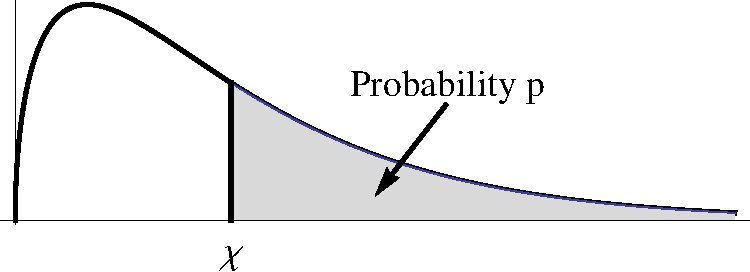
\includegraphics[width=.4\textwidth]{ChiPlot.pdf}
\sffamily
\scalefont{.5}
\begin{tabular}{|r|rrrrrrrrrr|}
\cline{2-11}
\multicolumn{1}{c}{\ }&\multicolumn{10}{|c|}{\small \scalefont{.65} p} \\
\hline \cellcolor{lightgray}	df	&\cellcolor{lightgray}	0.25	&\cellcolor{lightgray}	0.20	&\cellcolor{lightgray}	0.10	&\cellcolor{lightgray}	0.05	&\cellcolor{lightgray}	0.025	&\cellcolor{lightgray}	0.02	&\cellcolor{lightgray}	0.01	&\cellcolor{lightgray}	0.005	&\cellcolor{lightgray}	0.0025	&\cellcolor{lightgray}	0.001
\\ \hline	1	&	1.32	&	1.64	&	2.71	&	3.84	&	5.02	&	5.41	&	6.63	&	7.88	&	9.14	&	10.83
\\	2	&	2.77	&	3.22	&	4.61	&	5.99	&	7.38	&	7.82	&	9.21	&	10.60	&	11.98	&	13.82
\\	3	&	4.11	&	4.64	&	6.25	&	7.81	&	9.35	&	9.84	&	11.34	&	12.84	&	14.32	&	16.27
\\	4	&	5.39	&	5.99	&	7.78	&	9.49	&	11.14	&	11.67	&	13.28	&	14.86	&	16.42	&	18.47
\\	5	&	6.63	&	7.29	&	9.24	&	11.07	&	12.83	&	13.39	&	15.09	&	16.75	&	18.39	&	20.52
\\\cellcolor{lightgray}	6	&\cellcolor{lightgray}	7.84	&\cellcolor{lightgray}	8.56	&\cellcolor{lightgray}	10.64	&\cellcolor{lightgray}	12.59	&\cellcolor{lightgray}	14.45	&\cellcolor{lightgray}	15.03	&\cellcolor{lightgray}	16.81	&\cellcolor{lightgray}	18.55	&\cellcolor{lightgray}	20.25	&\cellcolor{lightgray}	22.46
\\\cellcolor{lightgray}	7	&\cellcolor{lightgray}	9.04	&\cellcolor{lightgray}	9.80	&\cellcolor{lightgray}	12.02	&\cellcolor{lightgray}	14.07	&\cellcolor{lightgray}	16.01	&\cellcolor{lightgray}	16.62	&\cellcolor{lightgray}	18.48	&\cellcolor{lightgray}	20.28	&\cellcolor{lightgray}	22.04	&\cellcolor{lightgray}	24.32
\\\cellcolor{lightgray}	8	&\cellcolor{lightgray}	10.22	&\cellcolor{lightgray}	11.03	&\cellcolor{lightgray}	13.36	&\cellcolor{lightgray}	15.51	&\cellcolor{lightgray}	17.53	&\cellcolor{lightgray}	18.17	&\cellcolor{lightgray}	20.09	&\cellcolor{lightgray}	21.95	&\cellcolor{lightgray}	23.77	&\cellcolor{lightgray}	26.12
\\\cellcolor{lightgray}	9	&\cellcolor{lightgray}	11.39	&\cellcolor{lightgray}	12.24	&\cellcolor{lightgray}	14.68	&\cellcolor{lightgray}	16.92	&\cellcolor{lightgray}	19.02	&\cellcolor{lightgray}	19.68	&\cellcolor{lightgray}	21.67	&\cellcolor{lightgray}	23.59	&\cellcolor{lightgray}	25.46	&\cellcolor{lightgray}	27.88
\\\cellcolor{lightgray}	10	&\cellcolor{lightgray}	12.55	&\cellcolor{lightgray}	13.44	&\cellcolor{lightgray}	15.99	&\cellcolor{lightgray}	18.31	&\cellcolor{lightgray}	20.48	&\cellcolor{lightgray}	21.16	&\cellcolor{lightgray}	23.21	&\cellcolor{lightgray}	25.19	&\cellcolor{lightgray}	27.11	&\cellcolor{lightgray}	29.59
\\	11	&	13.70	&	14.63	&	17.28	&	19.68	&	21.92	&	22.62	&	24.72	&	26.76	&	28.73	&	31.26
\\	12	&	14.85	&	15.81	&	18.55	&	21.03	&	23.34	&	24.05	&	26.22	&	28.30	&	30.32	&	32.91
\\	13	&	15.98	&	16.98	&	19.81	&	22.36	&	24.74	&	25.47	&	27.69	&	29.82	&	31.88	&	34.53
\\	14	&	17.12	&	18.15	&	21.06	&	23.68	&	26.12	&	26.87	&	29.14	&	31.32	&	33.43	&	36.12
\\	15	&	18.25	&	19.31	&	22.31	&	25.00	&	27.49	&	28.26	&	30.58	&	32.80	&	34.95	&	37.70
\\\cellcolor{lightgray}	16	&\cellcolor{lightgray}	19.37	&\cellcolor{lightgray}	20.47	&\cellcolor{lightgray}	23.54	&\cellcolor{lightgray}	26.30	&\cellcolor{lightgray}	28.85	&\cellcolor{lightgray}	29.63	&\cellcolor{lightgray}	32.00	&\cellcolor{lightgray}	34.27	&\cellcolor{lightgray}	36.46	&\cellcolor{lightgray}	39.25
\\\cellcolor{lightgray}	17	&\cellcolor{lightgray}	20.49	&\cellcolor{lightgray}	21.61	&\cellcolor{lightgray}	24.77	&\cellcolor{lightgray}	27.59	&\cellcolor{lightgray}	30.19	&\cellcolor{lightgray}	31.00	&\cellcolor{lightgray}	33.41	&\cellcolor{lightgray}	35.72	&\cellcolor{lightgray}	37.95	&\cellcolor{lightgray}	40.79
\\\cellcolor{lightgray}	18	&\cellcolor{lightgray}	21.60	&\cellcolor{lightgray}	22.76	&\cellcolor{lightgray}	25.99	&\cellcolor{lightgray}	28.87	&\cellcolor{lightgray}	31.53	&\cellcolor{lightgray}	32.35	&\cellcolor{lightgray}	34.81	&\cellcolor{lightgray}	37.16	&\cellcolor{lightgray}	39.42	&\cellcolor{lightgray}	42.31
\\\cellcolor{lightgray}	19	&\cellcolor{lightgray}	22.72	&\cellcolor{lightgray}	23.90	&\cellcolor{lightgray}	27.20	&\cellcolor{lightgray}	30.14	&\cellcolor{lightgray}	32.85	&\cellcolor{lightgray}	33.69	&\cellcolor{lightgray}	36.19	&\cellcolor{lightgray}	38.58	&\cellcolor{lightgray}	40.88	&\cellcolor{lightgray}	43.82
\\\cellcolor{lightgray}	20	&\cellcolor{lightgray}	23.83	&\cellcolor{lightgray}	25.04	&\cellcolor{lightgray}	28.41	&\cellcolor{lightgray}	31.41	&\cellcolor{lightgray}	34.17	&\cellcolor{lightgray}	35.02	&\cellcolor{lightgray}	37.57	&\cellcolor{lightgray}	40.00	&\cellcolor{lightgray}	42.34	&\cellcolor{lightgray}	45.31
\\	21	&	24.93	&	26.17	&	29.62	&	32.67	&	35.48	&	36.34	&	38.93	&	41.40	&	43.78	&	46.80
\\	22	&	26.04	&	27.30	&	30.81	&	33.92	&	36.78	&	37.66	&	40.29	&	42.80	&	45.20	&	48.27
\\	23	&	27.14	&	28.43	&	32.01	&	35.17	&	38.08	&	38.97	&	41.64	&	44.18	&	46.62	&	49.73
\\	24	&	28.24	&	29.55	&	33.20	&	36.42	&	39.36	&	40.27	&	42.98	&	45.56	&	48.03	&	51.18
\\	25	&	29.34	&	30.68	&	34.38	&	37.65	&	40.65	&	41.57	&	44.31	&	46.93	&	49.44	&	52.62
\\\cellcolor{lightgray}	30	&\cellcolor{lightgray}	34.80	&\cellcolor{lightgray}	36.25	&\cellcolor{lightgray}	40.26	&\cellcolor{lightgray}	43.77	&\cellcolor{lightgray}	46.98	&\cellcolor{lightgray}	47.96	&\cellcolor{lightgray}	50.89	&\cellcolor{lightgray}	53.67	&\cellcolor{lightgray}	56.33	&\cellcolor{lightgray}	59.70
\\\cellcolor{lightgray}	40	&\cellcolor{lightgray}	45.62	&\cellcolor{lightgray}	47.27	&\cellcolor{lightgray}	51.81	&\cellcolor{lightgray}	55.76	&\cellcolor{lightgray}	59.34	&\cellcolor{lightgray}	60.44	&\cellcolor{lightgray}	63.69	&\cellcolor{lightgray}	66.77	&\cellcolor{lightgray}	69.70	&\cellcolor{lightgray}	73.40
\\\cellcolor{lightgray}	50	&\cellcolor{lightgray}	56.33	&\cellcolor{lightgray}	58.16	&\cellcolor{lightgray}	63.17	&\cellcolor{lightgray}	67.50	&\cellcolor{lightgray}	71.42	&\cellcolor{lightgray}	72.61	&\cellcolor{lightgray}	76.15	&\cellcolor{lightgray}	79.49	&\cellcolor{lightgray}	82.66	&\cellcolor{lightgray}	86.66
\\\cellcolor{lightgray}	60	&\cellcolor{lightgray}	66.98	&\cellcolor{lightgray}	68.97	&\cellcolor{lightgray}	74.40	&\cellcolor{lightgray}	79.08	&\cellcolor{lightgray}	83.30	&\cellcolor{lightgray}	84.58	&\cellcolor{lightgray}	88.38	&\cellcolor{lightgray}	91.95	&\cellcolor{lightgray}	95.34	&\cellcolor{lightgray}	99.61
\\\cellcolor{lightgray}	80	&\cellcolor{lightgray}	88.13	&\cellcolor{lightgray}	90.41	&\cellcolor{lightgray}	96.58	&\cellcolor{lightgray}	101.88	&\cellcolor{lightgray}	106.63	&\cellcolor{lightgray}	108.07	&\cellcolor{lightgray}	112.33	&\cellcolor{lightgray}	116.32	&\cellcolor{lightgray}	120.10	&\cellcolor{lightgray}	124.84
\\\cellcolor{lightgray}	100	&\cellcolor{lightgray}	109.14	&\cellcolor{lightgray}	111.67	&\cellcolor{lightgray}	118.50	&\cellcolor{lightgray}	124.34	&\cellcolor{lightgray}	129.56	&\cellcolor{lightgray}	131.14	&\cellcolor{lightgray}	135.81	&\cellcolor{lightgray}	140.17	&\cellcolor{lightgray}	144.29	&\cellcolor{lightgray}	149.45 \\ \hline 

\end{tabular}
\end{center}
\end{minipage}
\end{center}

\end{document}